\chapter{Systematic Uncertainties}\label{ch:systematics}
Any measurement is affected by uncertainties that determine its range of validity. In this analysis, uncertainties are classified into various types: systematic errors related to the reconstructed objects, uncertainties arising from calculations of the cross-section, methodological errors, and statistical uncertainties. Each of these categories is explained in detail in the subsequent sections.

\section{Luminosity}
The combined integrated luminosity for the years 2015-2018 has an uncertainty of \qty[]{0.83}{\percent} determined with the LUCID-2 detector. It is applied to the Higgs Pair signal process and has minimal impact on this analysis.

\section{Jet Uncertainties}
Jets are calibrated using well known reference objects as described in section \ref{sec:calibration}. These corrections are themselves subject to uncertainties related to detector effects, modeling and statistics leading to corrections of the jet energy and are collectively referred to as \ac{jes} \citep{atlas2021jet,Aaboud:2019aa}. %Since simulations of jets have a higher accuracy than observed jets the uncertainties of the simulated jets are broadened to be consistent with the jets observed in the data.
Furthermore \ac{jer} uncertainties arise from the intrinsic resolution of the detector, noise and pileup contributions, and the algorithms used for jet reconstruction. In addition large-$R$ jets are corrected for their mass similar to the approach for the \ac{jes}. The uncertainties related to this procedure are called \ac{jmr} \citep{ATLAS-CONF-2020-022}. By the time of writing this thesis no calibrated uncertainties for large-$R$ jets were available for athena software release 24 used to  and thus uncertainties from a previous athena software release 21 \citep{Athena} serve as proxy uncertainties on the \ac{ufo} jets. This substitution is considered to be a minor limitation since the jet uncertainties play a minor role in this analysis as revealed by figure \ref{fig:jet_uncertainties}.
\begin{figure}
    \centering
    \subfigure[]{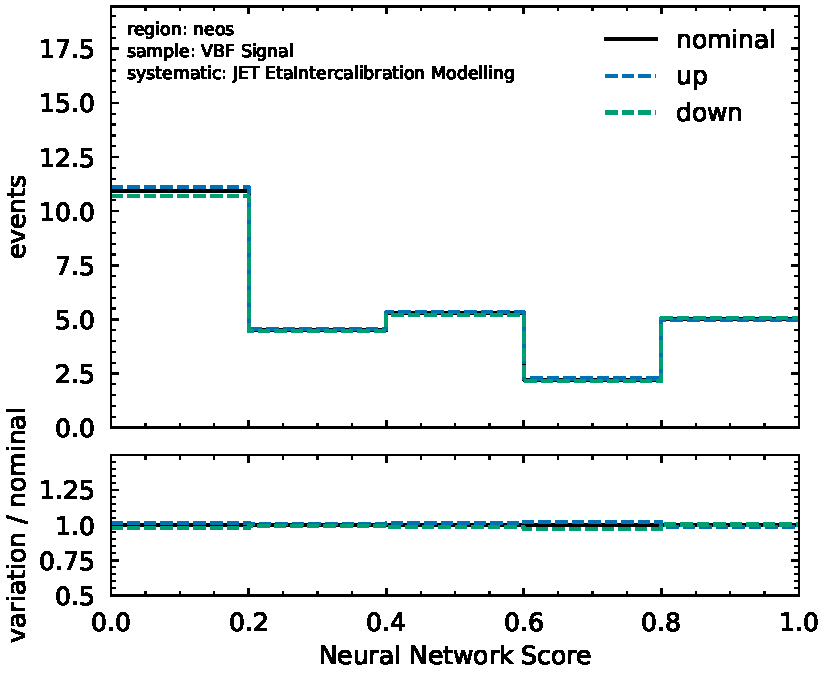
\includegraphics[width=.47\textwidth]{uncertainties/neos_VBF-Signal_JET-EtaIntercalibration-Modelling.pdf}}
    \subfigure[]{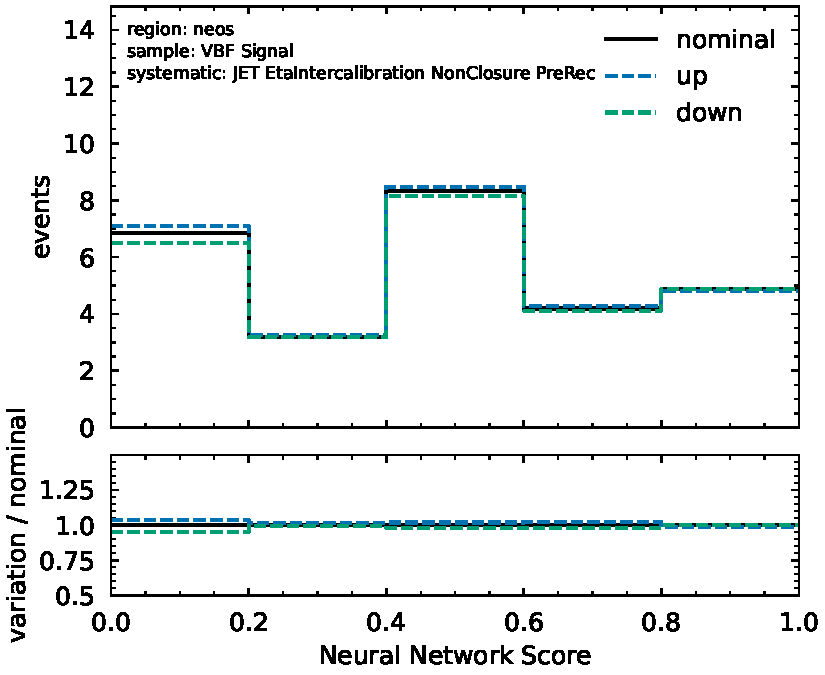
\includegraphics[width=.47\textwidth]{uncertainties/neos_VBF-Signal_JET-EtaIntercalibration-NonClosure-PreRec.pdf}}\\
    \subfigure[]{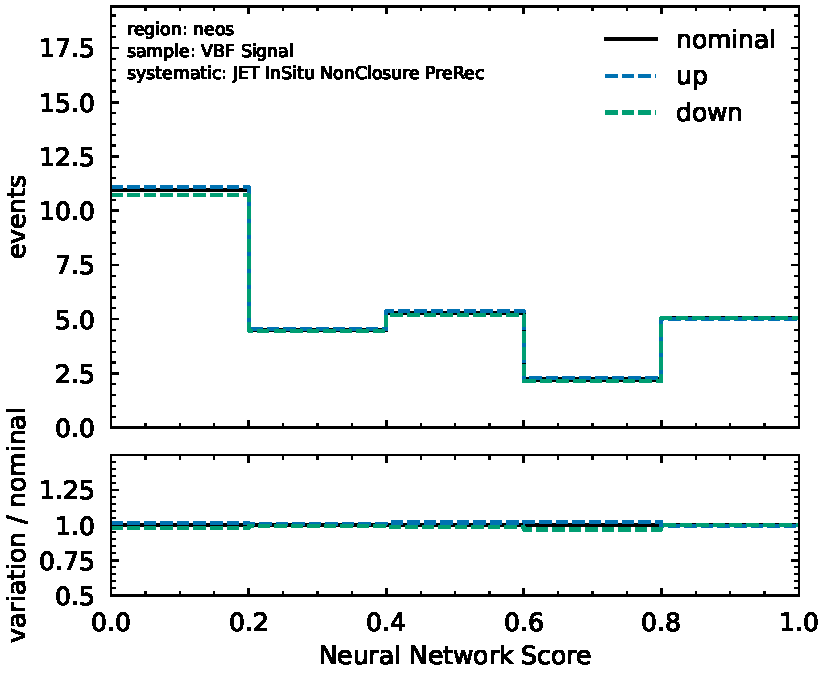
\includegraphics[width=.47\textwidth]{uncertainties/neos_VBF-Signal_JET-InSitu-NonClosure-PreRec.pdf}}
    \subfigure[]{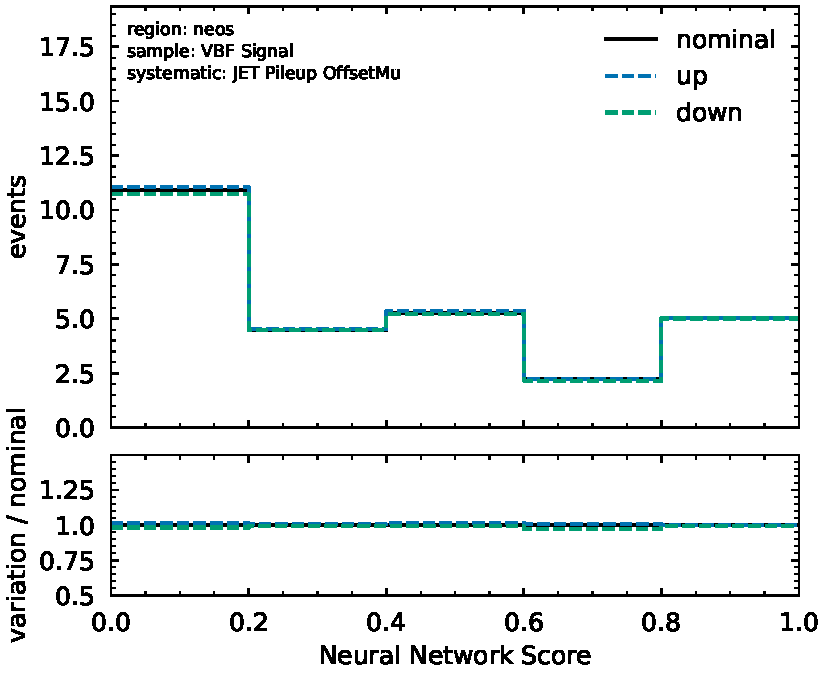
\includegraphics[width=.47\textwidth]{uncertainties/neos_VBF-Signal_JET-Pileup-OffsetMu.pdf}}\\
    \subfigure[]{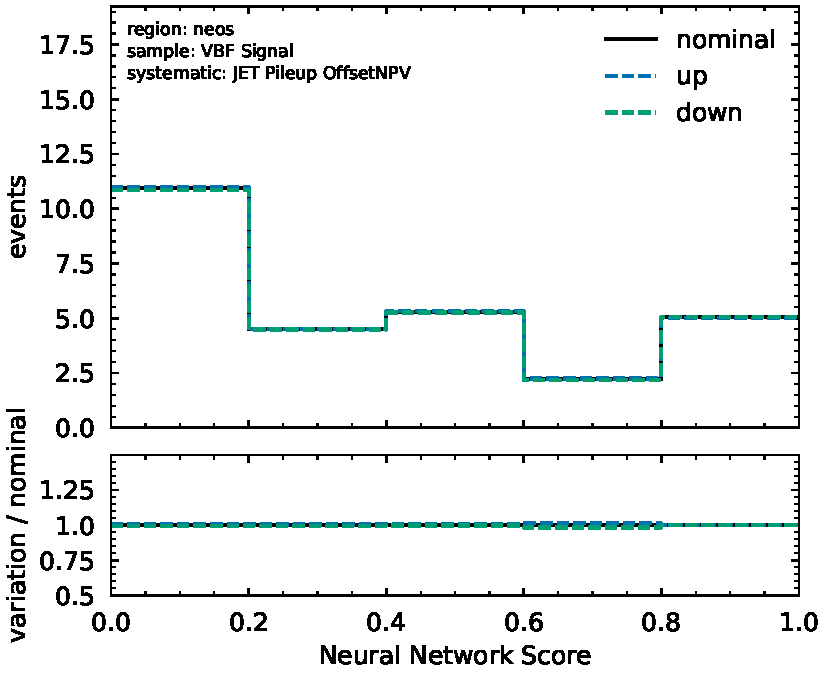
\includegraphics[width=.47\textwidth]{uncertainties/neos_VBF-Signal_JET-Pileup-OffsetNPV.pdf}}
    \subfigure[]{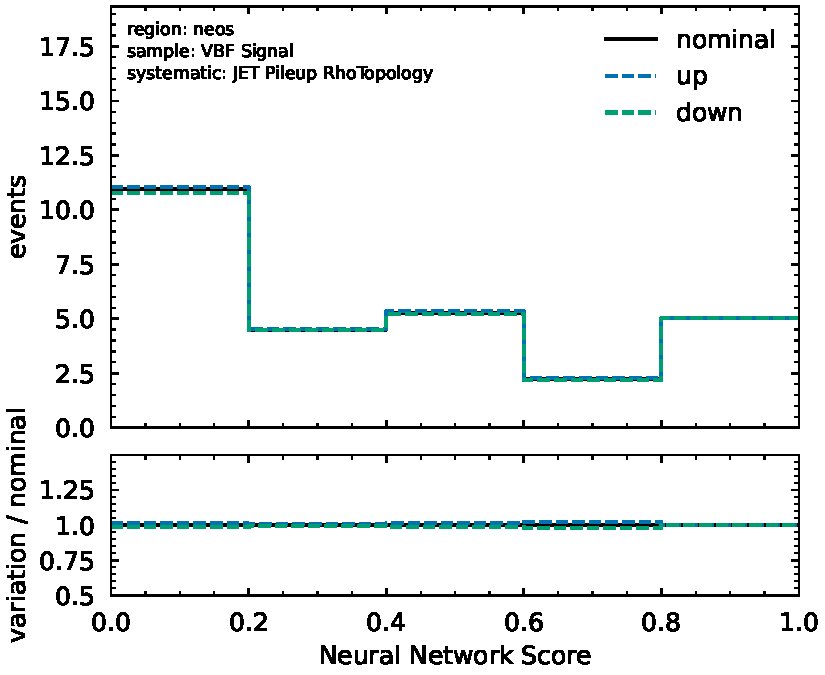
\includegraphics[width=.47\textwidth]{uncertainties/neos_VBF-Signal_JET-Pileup-RhoTopology.pdf}}
    \caption[]{Largest jet uncertainties on $\ktwov=0$ signal.}
    \label{fig:jet_uncertainties}
\end{figure}

f

\section{GN2X Tagger Uncertainties}
The training of the GN2X tagger uses simulations leading to potential discrepancies in selection efficiencies between observed data and simulation. These differences have not been estimated by the time of writing this thesis. It is assumed that the calibration will use the same procedure used by the previous version of this tagger - the $X\rightarrow bb$ tagger \citep{ATL-PHYS-PUB-2020-019}. This tagger was calibrated with $Z(\rightarrow b\overline{b})+\text{jets}$ and $Z(\rightarrow b\overline{b})+\gamma$ applying the same methodology as in \citep{ATL-PHYS-PUB-2021-035}. The differences between \ac{mc} and data are measured in large-$R$ jet \pt and the scale factors for the bins shown in figure \ref{fig:xbb_sf} are set to  $1\pm\qty[]{30}{\percent}$ as a proxy for the uncertainties and are shown in figure \ref{fig:xbb_uncertainties}. As in the previous iteration of this analysis these uncertainties are the dominating ones in this analysis.
\begin{figure}
    \centering
    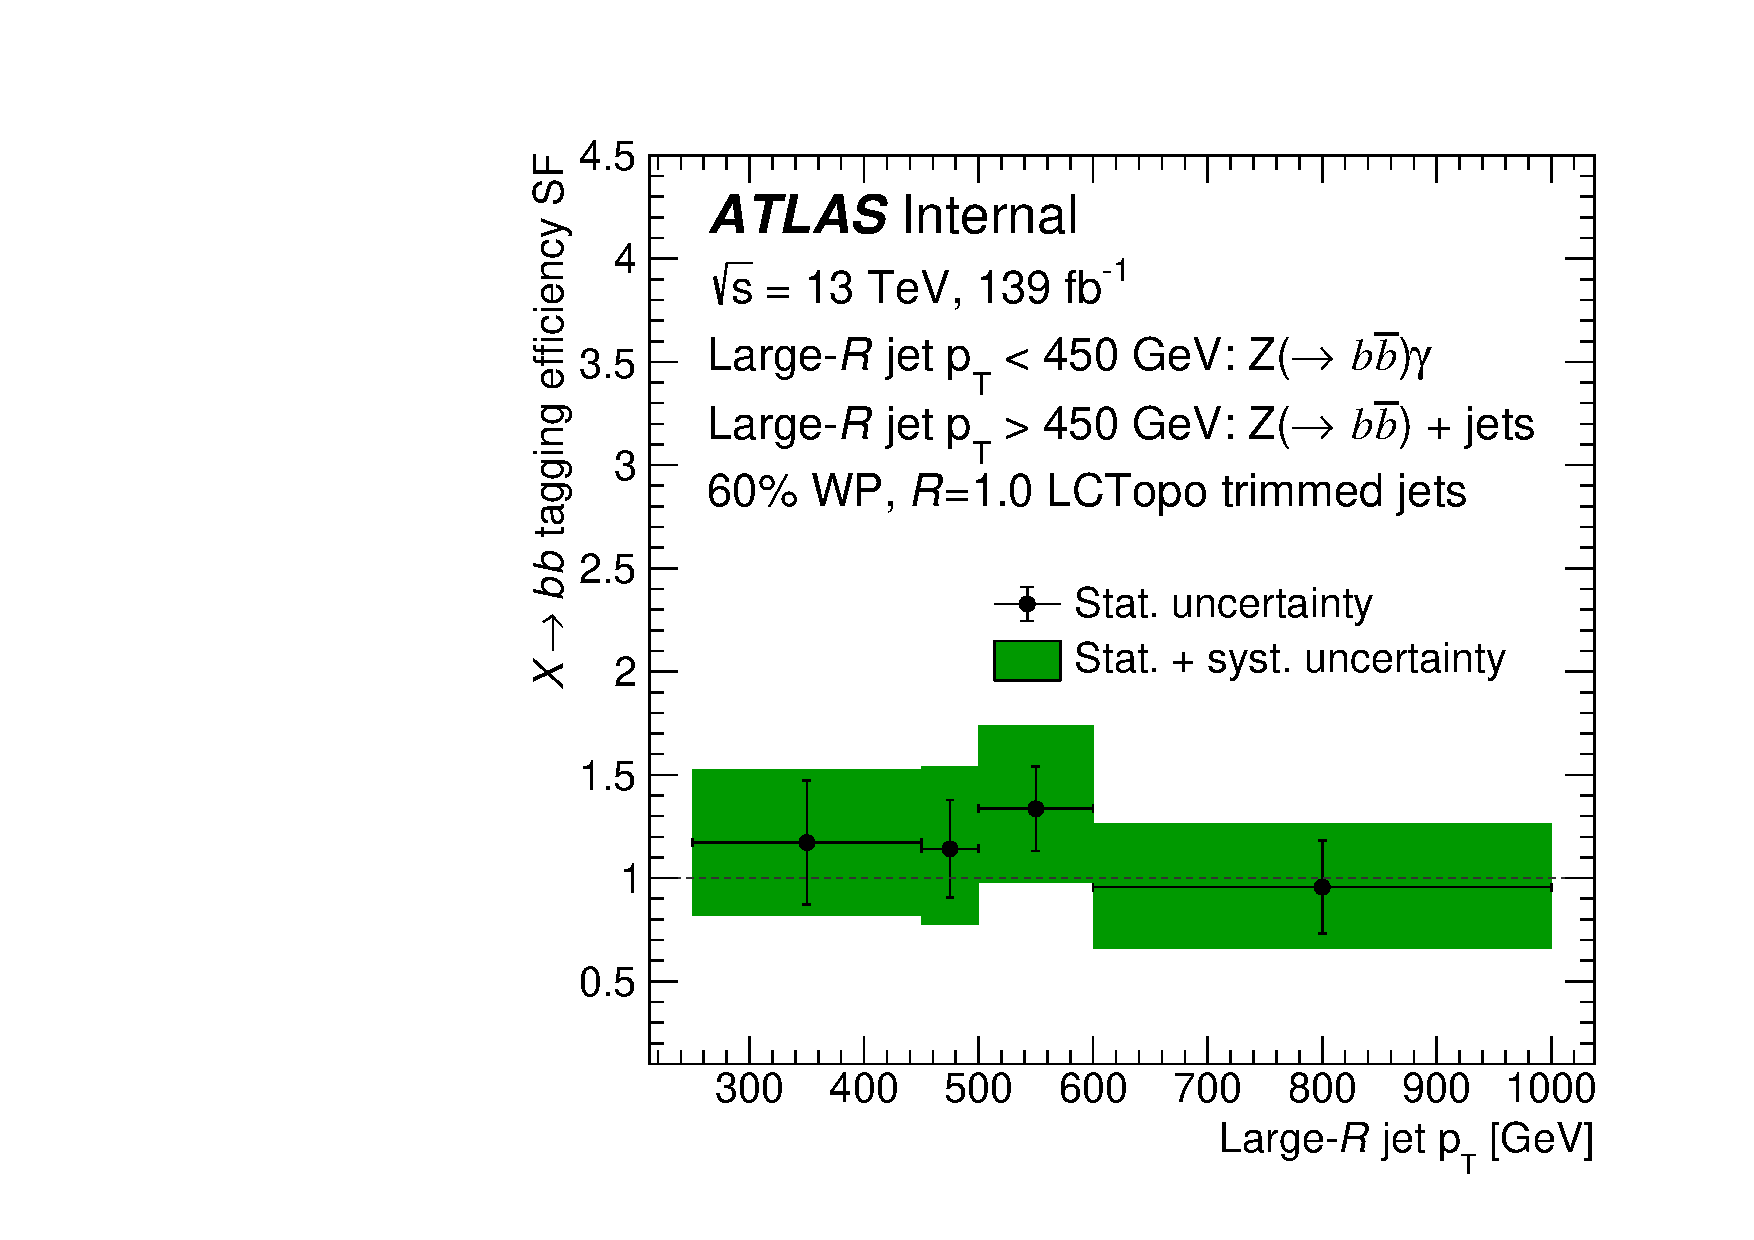
\includegraphics[width=.49\textwidth]{SF_Xbb60_internal_09March2023}
    \caption[]{Derived scale factors in large-$R$ jet \pt for the  \qty[]{60}{\percent} \ac{wp} from the calibration of the $X\rightarrow bb$ tagger.}
    \label{fig:xbb_sf}
\end{figure}

\begin{figure}
    \centering
    \subfigure[]{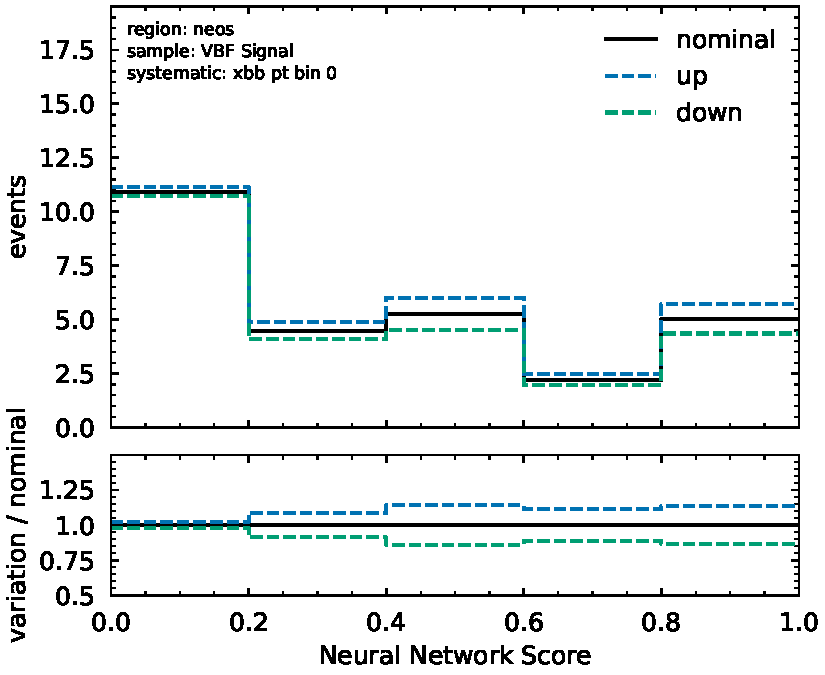
\includegraphics[width=.47\textwidth]{uncertainties/neos_VBF-Signal_xbb-pt-bin-0}}
    \subfigure[]{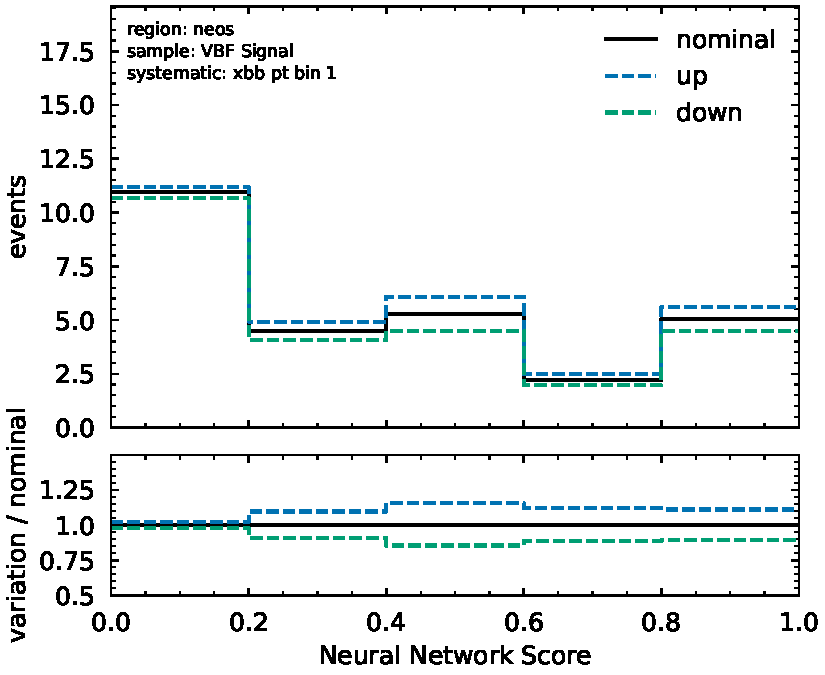
\includegraphics[width=.47\textwidth]{uncertainties/neos_VBF-Signal_xbb-pt-bin-1}}\\
    \subfigure[]{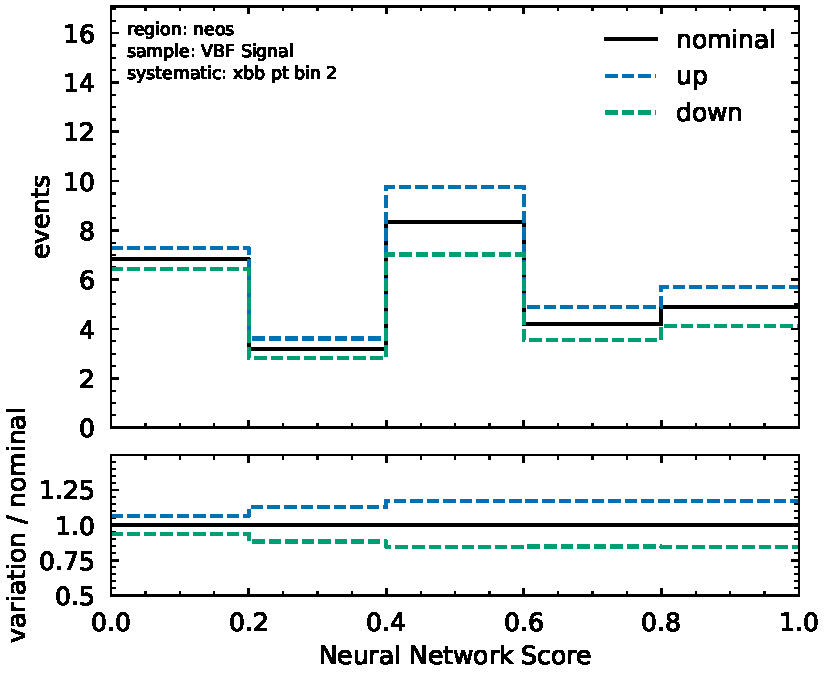
\includegraphics[width=.47\textwidth]{uncertainties/neos_VBF-Signal_xbb-pt-bin-2}}
    \subfigure[]{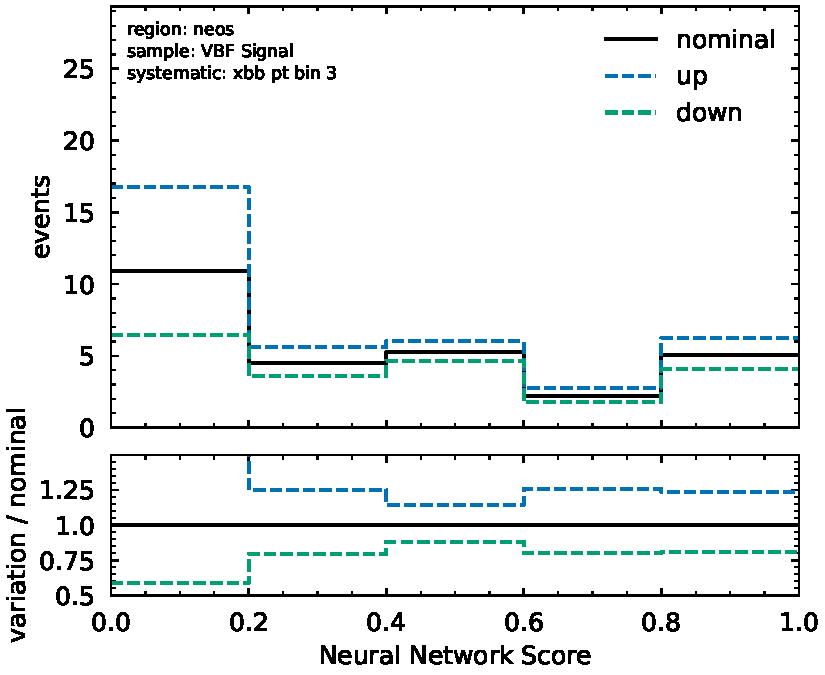
\includegraphics[width=.47\textwidth]{uncertainties/neos_VBF-Signal_xbb-pt-bin-3}}
    \caption[]{GN2X tagger uncertainties on the $\ktwov=0$ signal per scale factor bin from figure \ref{fig:xbb_sf}.}
    \label{fig:xbb_uncertainties}
\end{figure}



\section{Theory Uncertainties}\label{sec:theory_uncertainties}
The cross-section calculation for some process initiated by a proton proton collision calculated at $n$-th order as described in section \ref{sec:mc_simulation} has a functional form
\begin{equation}
    \sigma^{(n)} = PDF(x_1, \mu_F)  PDF(x_2, \mu_F) \hat{\sigma}^{(n)}(x_1,x_2,\mu_R),
    \label{eq:xs_unc_1}
\end{equation}
with the \acfp{pdf} carrying momentum fraction $x_{1,2}$ of the partons and the factorization scale $\mu_F$ \citep{unc_recipe}. The term $\hat{\sigma}^{(n)}$ in equation \ref{eq:xs_unc_1} is the calculable part of the cross-section at renormalization scale $\mu_R$ as described in section \ref{sec:renormalization}. This term is treated with the usual particles pyhsics \ac{qft} ansatz of expanding to a desired order $n$ in the strong coupling constant $\alpha_s$ as discussed in section \ref{sec:qft}
\begin{equation}
    \hat{\sigma}^{(n)} = \alpha_s \hat{\sigma}^{(0)} + \alpha_s^2 \hat{\sigma}^{(1)} + \ldots + \alpha_s^n \hat{\sigma}^{(n)} + \mathcal{O}(\alpha_s^{n+1}).
    \label{eq:xs_unc_2}
\end{equation}
Similar to renormalization a scaling behavior can be derived which allows to deduce an estimate of the \acp{pdf} by measuring it at some energy scale $\mu_F^2$ to extrapolate it to another. The equations enabling this are also expanded in $\alpha_s$ to a desired order and are known as DGLAP equations \citep{halzen1984introductory}. Three main sources of uncertainty arise in these calculations described in the following.

\subsection{Scale Variations}
$\alpha_s$ is expanded to some order $n$ in the cross-section calculation and as well in estimating the \acp{pdf}. To account for missing higher orders corrections of these expansions, scale variations of the renormalization and factorization scales are performed pairwise $\{\mu_\text{r},\mu_\text{f}\}\ \times \{0.5,0.5\}, \{1,0.5\}, \{0.5,1\}, \{1,1\}, \{2,1\}, \{1,2\}, \{2,2\}$. For the cross-section calculation this accounts essentially for the term $\mathcal{O}(\alpha_s^{n+1})$ in equation \ref{eq:xs_unc_2}. The envelope encompassing all scale variations is used as the uncertainty as depicted in figure \ref{fig:scale-variations}.


\subsection{\ac{pdf} + $\alpha_s$ Uncertainties}
\acp{pdf} need to be deduced from experiment and thus have experimental uncertainties. Further uncertainties arise from the functional forms assumed for the \acp{pdf}. $\alpha_s$ is  experimentally deduced at the scale of the $Z$ mass and therefore subject to uncertainties. In all perturbative calculations $\alpha_s$ is truncated at some order that needs to be accounted for \citep{unc_recipe,Butterworth_2016}.

The uncertainty introduced by the \acp{pdf} is calculated as a standard deviation of the cross section from the nominal \ac{pdf} set $\sigma^{(0)}$ \citep{Butterworth_2016}
\begin{equation}
    \Delta^\text{PDF}\sigma = \sqrt{\sum_k \left(\sigma^{(k)} - \sigma^{(0)}\right)^2}.
\end{equation}
The uncertainty on $\alpha_s=0.1180\pm0.0015$ is estimated with the associated uncertainty on $\alpha_s$ with
\begin{equation}
    \Delta^{\alpha_s}\sigma = \frac{\sigma(\alpha_s=0.1195)-\sigma(\alpha_s=0.1165)}{2}
\end{equation}
Since the correlation between $\alpha_s$ and the \acp{pdf} is small their uncertainties are applied quadratically combined \citep{unc_recipe,Butterworth_2016}.
\begin{equation}
    \Delta^{\text{PDF}+\alpha_s}\sigma=\sqrt{(\Delta^\text{PDF}\sigma )^2+(\Delta^{\alpha_s}\sigma)^2}
\end{equation}
The resulting shape uncertainties are shown in figure \ref{fig:pdf_alpha_s}.

\begin{figure}
    \centering
    \subfigure[]{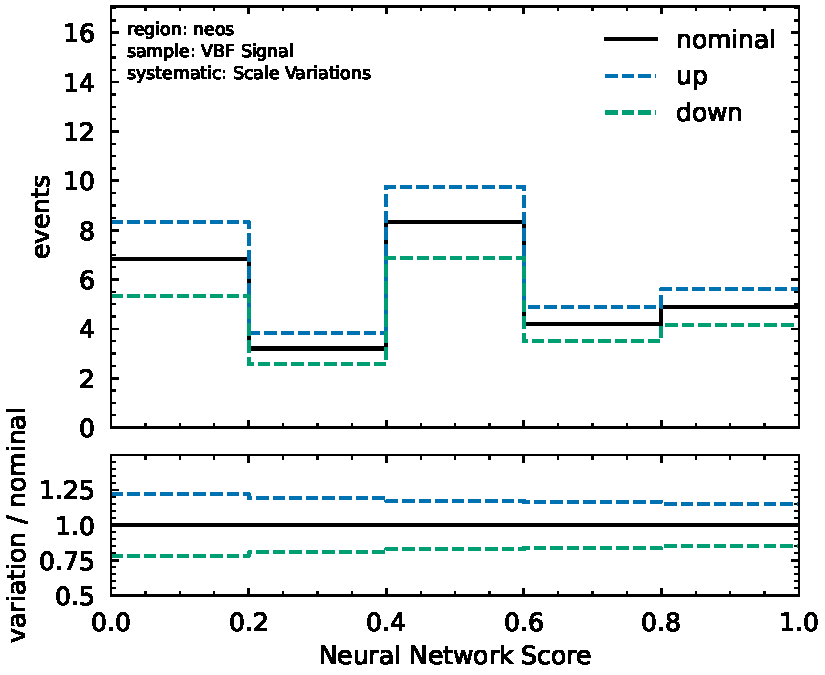
\includegraphics[width=.47\textwidth]{uncertainties/neos_VBF-Signal_Scale-Variations}
        \label{fig:scale-variations}
    }
    \subfigure[]{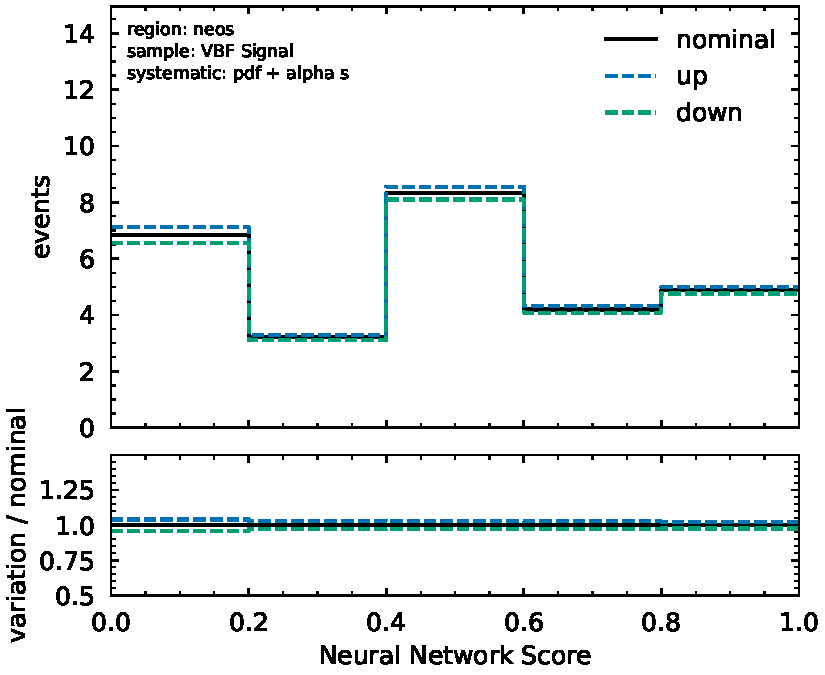
\includegraphics[width=.47\textwidth]{uncertainties/neos_VBF-Signal_pdf-+-alpha-s}
        \label{fig:pdf_alpha_s}    }
    \caption[]{$\ktwov=0$ signal uncertainties for \textbf{(a)} Scale variations and \textbf{(b)} \ac{pdf} + $\alpha_s$.}
    \label{fig:theory_unc}
\end{figure}

\subsection{Uncertainty on HH cross section}
Normalization uncertainties on the final acceptance are evaluated on \ac{mc} simulations for scale variations and for \acp{pdf} and $\alpha_s$. This is essentially a one bin normalization uncertainty of the theory uncertainties shown in figure \ref{fig:theory_unc}.

\subsection{Parton Shower}
Uncertainties related to the parton showering are estimated using different modelings from \textsc{Pythia 8} and \textsc{Herwig 7}. The largest deviations from the nominal are used as uncertainties on the Higgs pair process shown in figure \ref{fig:parton_shower}. This uncertainty is among the GN2X and scale variation uncertainties one of the dominating ones in this analysis.
\begin{figure}
    \centering
    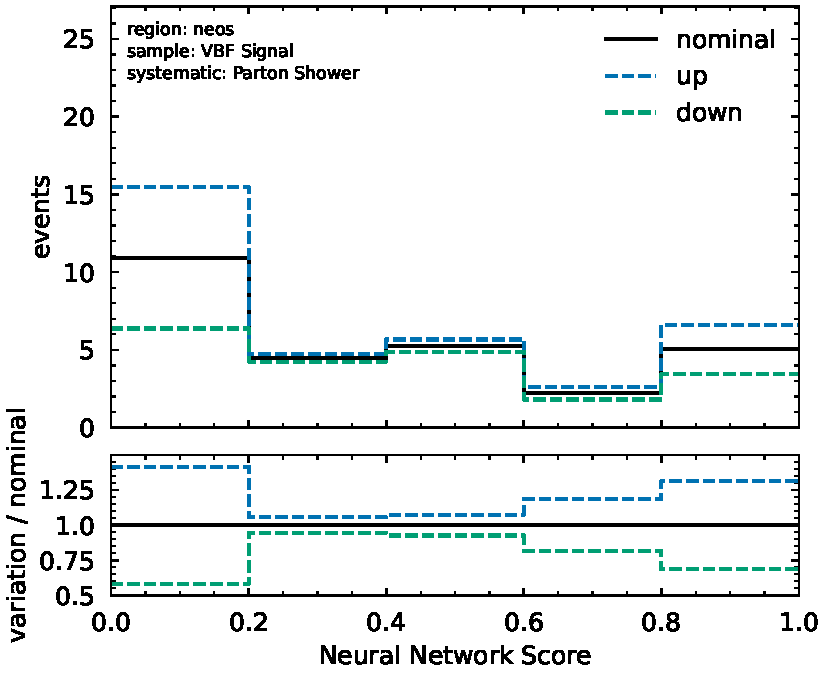
\includegraphics[width=0.7\textwidth]{uncertainties/neos_VBF-Signal_Parton-Shower}
    \caption[]{$\ktwov=0$ signal uncertainty for alternative parton shower with \textsc{Herwig 7}}
\end{figure}


\subsection{Branching Ratio Uncertainty}
The error estimate for the branching ratio takes into account theoretical uncertainties (THU) and parametric uncertainties (PU) that are included in the \ac{sm} calculations. The theoretical uncertainties mainly considers missing higher orders in the cross-section calculation, while for the parameters $p$ the four leading non-negligible uncertainty contributions of the strong coupling and the quark masses $p=\{\alpha_s,m_c,m_b,m_t\}$ are considered.

Parametric uncertainties are Gaussian errors and are added in quadrature which ensures unity in the Branching Ratio calculation \citep{de2016arxiv}. Theoretical uncertainties in turn are not Gaussian and would lead to underestimated errors and are therefore added linearly \citep{de2016arxiv}. By assuming a Higgs mass of \qty[]{125}{GeV} and considering that there are two Higgses decaying to two $b$-quarks the error on the branching ratio is
\begin{equation}
    \Delta\text{BR} = 2 \times \left(\Delta\text{BR}(\text{THU}) + \sqrt{\sum\nolimits_{p} \Delta\text{BR}(\text{PU}_{p})^2 }\right) = _{-3.5\%}^{+3.4\%}.
\end{equation}

\section{Statistical Uncertainties}
As discussed in chapter \ref{sec:statistics} on statistics the bin content for histograms in this work follows a Poisson distribution. Therefore the standard error for $N$ events is the square root of the Poisson variance $\sigma=\sqrt{\text{Var}}=\sqrt{N}$. Since histograms are filled weighted $\sum_i w_i N_i$ this needs to be taken into account. By making use of the additive property and invariance with respect to constants of the variance a bin filled with weights $w_i$ can be written as
\begin{align}
    \sigma_\text{stat}^2 & = \text{Var}_\text{bin}\left(\sum_i w_i\right)
    =
    \underbrace{\sum_i \text{Var}(w_i \times 1\text{ event})}_{\text{Var}(i+j)=\text{Var}(i)+\text{Var}(j)}
    =
    \underbrace{\sum_i w_i^2\text{Var}(1\text{ event})}_{\text{Var}(aX)=a^2\text{Var}(X)} \\ \nonumber
                         & =\sum_i w_i^2\sqrt{(1\text{ event})},
\end{align}
so that the statistical error reads
\begin{equation}
    \sigma_\text{stat}^\text{bin}=\sqrt{\sum_i w_i^2}.
\end{equation}

\section{Background Derivation Uncertainties}\label{sec:bkg_uncertainties}
\red{add bounding}
The \ac{qcd} background is estimated with the ABCD method from the control region as detailed in section \ref{sec:abcd}. The uncertainties on the weight factor $w_\text{CR}$ are assessed through error propagation of the statistical uncertainties on the quantities used to calculate the weight
\begin{equation}
    \Delta_\text{stat} w_\text{CR} = w_\text{CR} \sqrt{
        \left(\frac{\Delta_\text{stat} N_\text{CR}^\text{2 GN2X}}{N_\text{CR}^\text{2 GN2X}}\right)^2
        +
        \left(\frac{\Delta_\text{stat} N_\text{CR}^\text{1 GN2X}}{N_\text{CR}^\text{1 GN2X}}\right)^2
    }
    = \red{\qty[]{8.3}{\percent}}.
\end{equation}
To estimate the uncertainty of the background estimate in the \ac{sr} a shape uncertainty is estimated from the \ac{vr} by symmetrizing about the difference between the estimate, and the selection with 2 GN2X tags
\begin{equation}
    \Delta_\text{shape}^\text{bkg}= \left| w_\text{CR}N_\text{VR}^\text{1 GN2X} - N_\text{VR}^\text{2 GN2X}\right|.
\end{equation}
Figure \ref{fig:bkg_shape_estimate} displays the background estimate in the \ac{vr} in comparison to the \ac{vr} with 2 GN2X tags and the resulting shape uncertainty in the \ac{sr}.
\begin{figure}
    \centering
    \subfigure[]{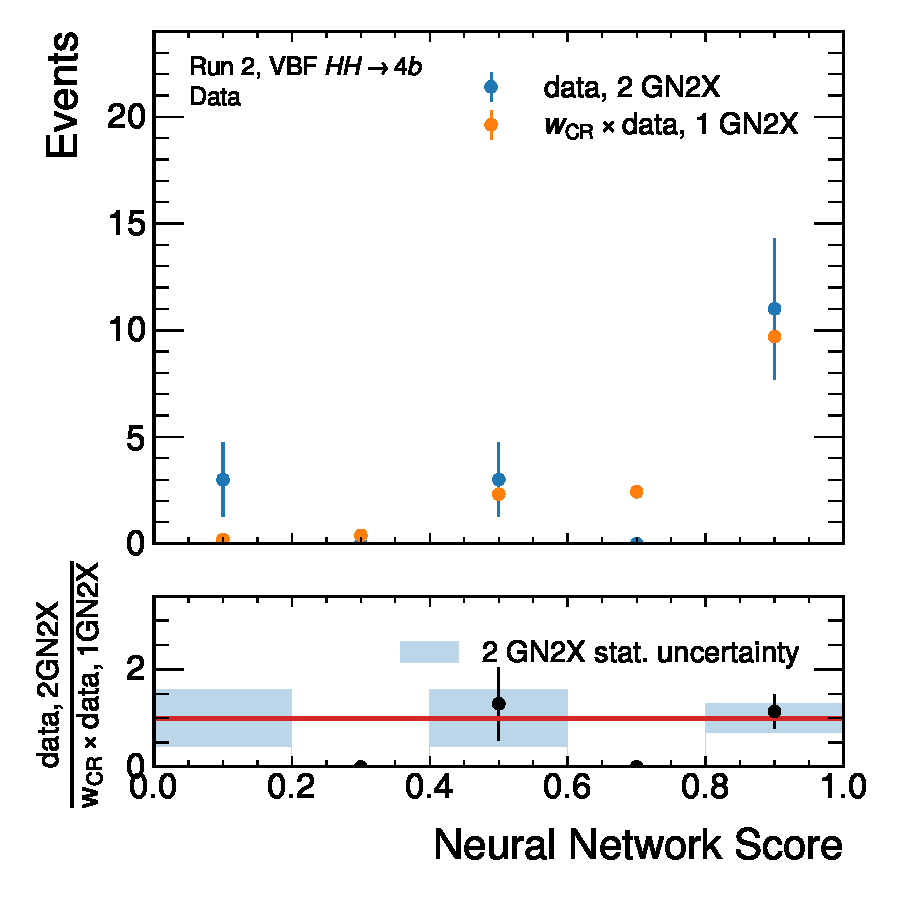
\includegraphics[width=.47\textwidth]{tomatos_cls_5_2500_slope_50_NOSYS.VR_xbb_2_compareABCD}}
    \subfigure[]{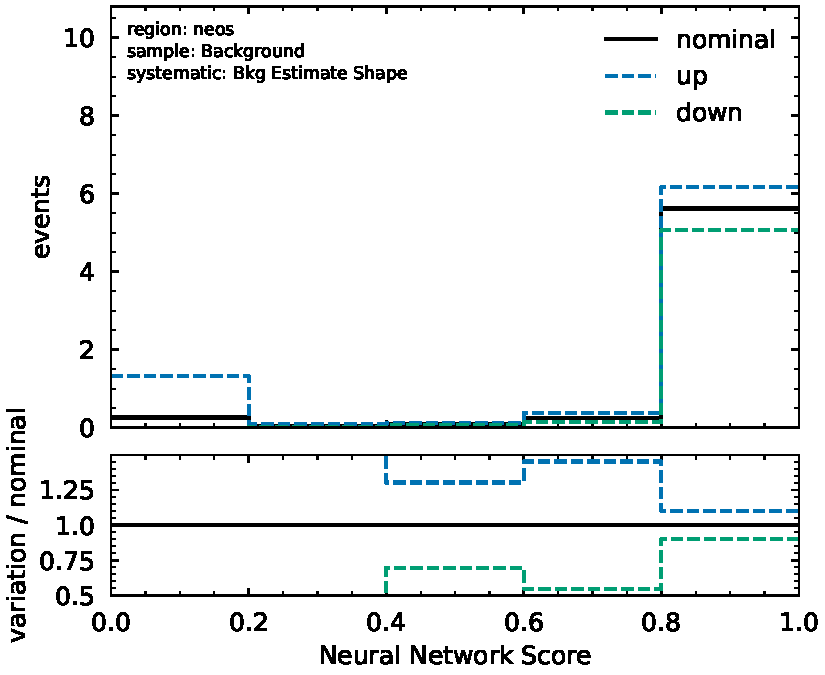
\includegraphics[width=.47\textwidth]{neos_results/neos_Background_Bkg-Estimate-Shape}}
    \caption[]{(a) Background estimate in the \ac{vr} in comparison to the the selection with 2 GN2X tags. (b) Extracted uncertainties from (a) applied to the background estimate in the \ac{sr}.}
    \label{fig:bkg_shape_estimate}
\end{figure}

